% Template for ICASSP-2027 paper; to be used with:
%          spconf.sty  - ICASSP/ICIP LaTeX style file, and
%          IEEEbib.bst - IEEE bibliography style file.
% --------------------------------------------------------------------------
\documentclass{article}
\usepackage{spconf,amsmath,amssymb,graphicx,multirow,booktabs}
\usepackage{tabularx}
\usepackage[hidelinks]{hyperref}
\usepackage{orcidlink}
\usepackage{balance} % balance the two columns on the last (references) page

% 排版紧凑化（图表与正文间距 + section 标题间距）
\setlength{\textfloatsep}{4.5pt plus 1.5pt minus 1.5pt}
\setlength{\floatsep}{4.5pt plus 1.5pt minus 1.5pt}
\setlength{\dbltextfloatsep}{4.5pt plus 1.5pt minus 1.5pt}
\usepackage{titlesec}
\titlespacing*{\section}{0pt}{1.0ex plus 0.3ex minus 0.2ex}{0.6ex plus 0.2ex}
\titlespacing*{\subsection}{0pt}{0.6ex plus 0.2ex}{0.4ex plus 0.1ex}
% 公式紧凑化（版面预算）
\setlength{\abovedisplayskip}{3pt plus 1pt minus 1pt}
\setlength{\belowdisplayskip}{3pt plus 1pt minus 1pt}

% Custom commands
% —— 记号规范（师兄整改）：标量斜体 / 向量粗小写 \mathbf{z} / 矩阵粗大写 \mathbf{X} / 集合花体 \mathcal{T} / 算子正体 \operatorname；f 专用于模型函数，频率 bin 索引用 m
\DeclareMathOperator{\EER}{EER}
\DeclareMathOperator{\AUC}{AUC}
\DeclareMathOperator{\Do}{do}
\newcommand{\dEER}{\Delta\EER}

% Title.

\title{Objective Alignment for Faithful Attribution in Speaker Verification}
% ---- 作者与机构信息 ----
\name{Xiaolei Zhang\,\orcidlink{0009-0006-2263-6044}$^{1}$ \qquad Zhihua Fang\,\orcidlink{0000-0002-3018-7414}$^{2}$ \qquad Zhe Li\,\orcidlink{0000-0002-0519-7434}$^{3}$ \qquad Xiaoxiao Miao\,\orcidlink{0000-0002-6645-6524}$^{4}$ \qquad Liang He\,\orcidlink{0000-0003-4076-7479}$^{2,5 \star}$\thanks{$^{\star}$Corresponding author (heliang@mail.tsinghua.edu.cn). This work was supported by the National Natural Science Foundation of China (No.\ 62366051).}}
\address{
  $^{1}$School of Software, Xinjiang University, China \\
  $^{2}$School of Computer Science and Technology, Xinjiang University, China \\
  $^{3}$Speech, Language, and Cognition Laboratory, The University of Hong Kong, Hong Kong SAR, China \\
  $^{4}$Duke Kunshan University, China \\
  $^{5}$Department of Electronic Engineering, Tsinghua University, China \\
}

\begin{document}
%\ninept
%
\maketitle
%
% ========================================================================
% 摘要：钩子前置（归因可信取决于目标）→ 两轨统一 → 目标受控变量 → 两阶段 → 应用（师兄改版配套微调）
% ========================================================================
\begin{abstract}
% 【中文】归因可信与否不仅取决于算法，也取决于被解释的目标。说话人验证（SV）的可解释性沿两条几乎不相交的路径发展：归因（哪些帧驱动了判决）与语言学先验（哪些音素类承载说话人信息）。二者构建于不同协议之上，很少相互印证。我们用\emph{帧干预}将其统一：置零选定的帧集合、测量 EER 的变化，两条轨道仅在"如何选帧"上不同。在这一视角下，我们把归因\emph{目标函数}当作受控变量，在判别性/表征性双重忠实度指标下比较四种算法 × 三种目标。将目标对齐到验证判决可以提升每一种算法的忠实度，但其提升幅度强烈依赖于算法——对 CAM 类方法显著、对梯度类方法可忽略——揭示出一种结构化的"目标×算法"交互，而非某个单一主导因素。把由此得到的忠实归因应用到五个仅在数据增强上不同的 ECAPA-TDNN 模型上，我们将 SpecAug 与最大的音素依赖重塑关联起来，并观察到归因与干预两条轨道导出的音素排序一致：元音类在两条轨道中都居首。
Whether an attribution for speaker verification (SV) can be trusted depends not only on the algorithm but on the objective it explains. SV interpretability has advanced along two tracks that rarely meet: attribution, which asks which frames drive a decision, and linguistic priors, which ask which phonetic classes carry speaker information. We unify them under \emph{frame intervention}: zero a chosen frame set and measure the change in EER, the two tracks differing only in how frames are selected. Under this protocol, we treat the attribution \emph{objective} as a controlled variable and compare four algorithms across three objectives with discriminative and representational faithfulness metrics. Objective alignment has a clear two-stage structure: removing the norm improves faithfulness for every algorithm, whereas the further step to the paired form is algorithm-dependent, aiding CAM-based methods substantially and gradient-based ones only marginally. Applied to five ECAPA-TDNN models differing in augmentation or training strategy, the framework associates SpecAug with the largest reshaping of phoneme dependency, and the attribution- and intervention-derived phoneme rankings agree: the vowel class ranks foremost in both tracks.
\end{abstract}
%
\begin{keywords}
Speaker verification, interpretability, attribution, phoneme, faithfulness
\end{keywords}
%
% ========================================================================
% §1 引言（师兄改版六段）：问题张力 → objective 是被忽视的变量 → 帧干预+双指标 → 两阶段结构 → 训练策略重塑音素 → 贡献列表
% Related Work 折入 P2/P3/P5 引文（无独立 Related Work 一节）；贡献用 itemize
% ========================================================================
\section{Introduction}
\label{sec:intro}

% P1【中文】SV 基准不断提升，但模型依据哪些声学证据做判决仍未解决；后验归因给输入帧/时频区域赋重要性作答。归因可信与否不仅取决于解释算法，还取决于被解释目标是否与模型真实执行的判决一致。SV 尤其如此——它不是固定类分类，而是依据两个表征相似度与阈值的开放集成对判断；解释分类 logit、嵌入范数或单一相似度，不必然等于解释验证判决。
Deep speaker verification (SV) systems~\cite{ECAPATDNNEmphasizedChannel2020a} keep improving on standard benchmarks, yet a more basic question remains open: on what acoustic evidence does a model base its verification decisions? Post-hoc attribution answers this by assigning importance to frames or time--frequency regions, but whether an attribution can be trusted depends not only on the explanation algorithm---it also depends on whether the explained objective matches the decision the model actually executes. SV is not classification over fixed classes but an open-set pairwise judgment on the similarity between two representations and a threshold, so explaining a classification logit, an embedding norm, or a single similarity does not necessarily explain the verification decision itself.

% P2【中文】既有 SV 归工作或固定单一目标只变算法：IG 作用于嵌入 L2 范数、CAM 系于识别目标下比较、Thébaud 单余弦+IG 未量化忠实度；attribution objective 本身成为被系统忽视的变量。从 SV 判决结构看不同目标与真实验证过程距离不同：嵌入 L2 范数仅描述表征幅值，同说话人余弦进一步引入参考语音，同+异说话人成对余弦差直接对应验证 margin。核心问题：随归因目标逐步对齐真实验证判决，忠实度是否系统提高？独立于算法还是与算法交互？
Existing SV interpretability studies focus on the attribution \emph{algorithm} while fixing one pre-selected objective: Integrated Gradients (IG) on the embedding L2 norm~\cite{zhang2023visualizing}, CAM variants (Grad-CAM, LayerCAM, Score-CAM) compared under identification objectives~\cite{li2022reliable,li2024phonemes}, or a same-speaker cosine without quantified faithfulness~\cite{thebaud2024phonetic}. The attribution \emph{objective} itself is thereby left unexamined, although candidate objectives sit at different distances from the verification process: the embedding L2 norm describes only the magnitude of the representation, the same-speaker cosine adds a reference utterance, and the paired cosine difference over same- and different-speaker references corresponds directly to the verification margin. Does systematically aligning the objective with the verification decision improve faithfulness---independently of the algorithm, or interacting with it?

% P3【中文】需要不依赖具体目标的忠实度评价。统一帧干预协议：归因选出帧、置零、重提嵌入、重打分（同通用 XAI 删除式评估，SV 此前仅服务识别目标）；EER 变化不完备——同/异得分可能共移，表征明显受损而 EER 变化不大；判别忠实度看是否改变最终验证性能，表征忠实度看是否破坏目标与同说话人参考的表征一致性。
Answering this calls for a faithfulness measure independent of the chosen objective. We adopt a unified \emph{frame intervention} protocol---the same deletion-based idea as in general XAI~\cite{petsiuk2018rise,deyoung2020eraser}, so far applied in SV only to identification objectives: an attribution selects frames, they are zeroed, embeddings re-extracted, and trials re-scored. EER change alone, however, does not fully describe faithfulness: same- and different-speaker scores may shift together, so a representation can be visibly damaged while the EER barely moves. We therefore evaluate attribution at two complementary levels: \emph{discriminative faithfulness}, whether intervention changes the final verification performance, and \emph{representational faithfulness}, whether intervention destroys the target's agreement with a same-speaker reference.

% P4【中文】实验表明 objective alignment 不是简单的越对齐越好，而呈两阶段结构：L2→cosine（从表征幅值到验证几何）一致提升全部四算法的判别忠实度；cosine→paired（加异说话人参考）则显著依赖算法——CAM 系大升、梯度系微变。归因忠实度由目标×算法交互决定。
Experiments show that objective alignment is not a simple monotone: it exhibits a two-stage structure. Replacing the L2 norm by cosine similarity---from representation magnitude toward the verification geometry---consistently improves discriminative faithfulness for all four algorithms; the further step from single to paired cosine is strongly algorithm-dependent: CAM-based methods gain substantially, whereas gradient-based methods change little---faithfulness is set by the objective--algorithm interaction, not by either alone.

% P5【中文】更实质的模型行为问题：不同训练策略是否改变模型所依赖的语音学信息？五个共享 ECAPA-TDNN、仅数据增强/训练策略不同的模型上对元音/塞音/鼻音/擦音/流音做类别级干预；训练策略不仅改变 EER，也显著改变信息使用模式，SpecAug 关联最明显的重塑且集中于元音；两条独立分析路径（归因重要性排序 vs 干预 ΔEER 排序）均将元音置于首位——归因结果的跨路径一致性检验。
With faithful configurations established, we use the same framework to ask whether different training strategies change the phonetic information an SV model relies on---a question left open by prior work on which phonetic classes carry speaker information~\cite{li2024phonemes,benamor2023describing} or on phonetic-knowledge injection into representations~\cite{liu2019phonetic,song2024multilingual,ma2025phinet}. Across five models sharing the ECAPA-TDNN architecture and differing only in augmentation or training strategy, we perform class-level interventions on vowels, plosives, nasals, fricatives, and liquids. Training strategy reshapes more than the EER---it alters which information the model uses, with SpecAug associated with the largest reshaping, concentrated in the vowel class. Two independent paths---the saliency-derived importance ranking and the intervention-derived $\dEER$ ranking---both place the vowel class foremost, a cross-path consistency check.

% P6【中文贡献1】objective 作为独立设计变量：表征级 L2 范数→相似度级余弦→判决级成对目标的系统对齐比较
% 【中文贡献2】统一帧干预评价框架+判别/表征双指标：区分真实不忠实与 EER 共移效应
% 【中文贡献3】4 算法×5 训练条件：objective–algorithm 交互所致两阶段规律；训练策略系统性重塑音素依赖，元音在归因与干预两轨均居首
This paper makes three contributions:
\begin{itemize}
  \item \textbf{Attribution objective as a design variable}: a systematic comparison of objective alignment from the representation-level L2 norm, through the similarity-level cosine, to the decision-level paired target.
  \item \textbf{A unified frame-intervention framework for faithfulness}: frame zeroing with discriminative and representational metrics, separating true unfaithfulness from the EER co-shift artifact.
  \item \textbf{Two-stage alignment and training-induced reshaping}: across four algorithms and five training conditions, a two-stage law from the objective--algorithm interaction, and evidence that training strategy reshapes phoneme dependency---vowel foremost in both tracks.
\end{itemize}

% ========================================================================
% §2 方法（记号体系统一，师兄整改）：2.1 形式化与记号 → 2.2 归因目标 → 2.3 帧级归因与干预 → 2.4 忠实度评价 → 2.5 音素级干预与跨轨一致性
% ========================================================================
\section{Methodology}
\label{sec:framework}

\subsection{Problem Formulation and Notation}

% 【中文】记号规范：标量斜体、向量粗小写、矩阵粗大写、集合花体、算子正体。f_θ 映 F×T 维 log-mel 输入 X 到 D 维嵌入 z=f_θ(X)；验证对两个嵌入间的余弦加阈值，以同/异说话人参考 X⁺,X⁻ 及其嵌入 z⁺,z⁻，margin s(X)=cos(z,z⁺)−cos(z,z⁻) 捕获验证判决，EER 由诱导出的同/异得分分布的可分离度决定。
Scalars are set in italics, vectors in bold lowercase, matrices in bold uppercase, sets in calligraphic capitals. An SV model $f_{\theta}:\mathbb{R}^{F\times T}\to\mathbb{R}^{D}$ maps an $F$-bin log-mel input $\mathbf{X}\in\mathbb{R}^{F\times T}$ of $T$ frames to a $D$-dimensional embedding $\mathbf{z}=f_{\theta}(\mathbf{X})$. Verification thresholds the cosine between two embeddings; with same- and different-speaker references $\mathbf{X}^{+},\mathbf{X}^{-}$ and their embeddings $\mathbf{z}^{+},\mathbf{z}^{-}$, the margin function $s(\mathbf{X})=\cos(\mathbf{z},\mathbf{z}^{+})-\cos(\mathbf{z},\mathbf{z}^{-})$ captures the verification decision, and the $\EER$ is set by the separability of the induced same- and different-speaker score distributions.

\subsection{Attribution Objectives}

% 【中文】三目标按与验证判决对齐程度排序：表征级 g_ℓ2=‖z‖₂（Li 所用）、相似度级 g_cos=cos(z,z⁺)、判决级 g_pc=s(X)（重合 margin）；IG/LayerCAM/Score-CAM/Guided IG 四算法对三目标逐一评估。
We compare three attribution objectives ordered by how tightly they match the verification decision: the representation-level norm $g_{\ell_2}(\mathbf{X})=\|\mathbf{z}\|_2$ used by Li et al.~\cite{zhang2023visualizing}, the similarity-level same-speaker cosine $g_{\cos}(\mathbf{X})=\cos(\mathbf{z},\mathbf{z}^{+})$, and the decision-level paired form $g_{\mathrm{pc}}(\mathbf{X})=s(\mathbf{X})$, coinciding with the margin function. We evaluate four algorithms against all three objectives: IG~\cite{sundararajan2017axiomatic}, LayerCAM~\cite{jiang2021layercam}, Score-CAM~\cite{wang2020scorecam}, and Guided IG~\cite{kapishnikov2021guided}.

\subsection{Frame-level Attribution and Intervention}

% 【中文】两条可解释性轨道都归结为选帧集合 𝒯：对全部频 bin 置零、重提嵌入、重打分、报 ΔEER(𝒯)；只干预目标句，参考嵌入 z⁺,z⁻ 恒由完整输入算得，故归因解释的是目标句对成对判决的贡献。归因方法给目标句一张显著图 A∈R^{F×T}，按各方法符号语义聚合为逐帧重要性 φ_t（IG 系 |a|，CAM 系 ReLU）；归因轨取 top-k 帧，置零/重嵌入/重打分两轨全同。
Both interpretability tracks reduce to selecting a frame index set $\mathcal{T}\subseteq\{1,\ldots,T\}$: zero the entries $X_{m,t}$ of $\mathbf{X}$ for $t\in\mathcal{T}$ over all frequency bins $m\in\{1,\ldots,F\}$, recompute the embeddings, re-score the trial set, and report $\dEER(\mathcal{T})=\EER(\mathcal{T})-\EER_{\mathrm{base}}$. Only the target utterance is intervened on; reference embeddings are always computed from intact input, so attribution explains the target's contribution to the paired decision. An attribution method assigns the target utterance a saliency map $\mathbf{A}\in\mathbb{R}^{F\times T}$, which is aggregated to a per-frame importance by a rule matched to each method's sign semantics,
\begin{equation}
  \phi_t = \begin{cases} \sum_{m} |A_{m,t}|\,, & \text{IG, Guided IG}\,, \\[1pt] \sum_{m} \mathrm{ReLU}\!\left(A_{m,t}\right)\,, & \text{CAM methods}\,. \end{cases}
  \label{eq:phi}
\end{equation}
The attribution track takes $\mathcal{T}$ as the top-$k$ frames under $\phi_t$; zeroing, re-embedding, and re-scoring are identical across tracks---only the source of $\mathcal{T}$ differs.

\subsection{Faithfulness Evaluation}
\label{sec:faith}

% 【中文】EER 是可分离度度量，删除可能让同/异得分同移(co-shift)，是真不忠实与共移遮蔽的混淆源；判别性指标=梯形积分归一化 EER 曲线 e(r)；表征性指标=同说话人保持率 ρ(r)=s̄(r)/s̄_base（免共移）；二者联合判断干预是否既改变判决又破坏表征。
Since $\EER$ is a separability metric, deleting important frames may shift same- and different-speaker scores together and leave $\EER$ nearly unchanged: a co-shift artifact of the verification decision function. To separate genuine unfaithfulness from this masking, we report two complementary metrics over a frame-ratio sweep $\mathcal{R}$ of $K{=}13$ points between $0.05$ and $0.90$. The \emph{discriminative} metric follows the ranking induced by Eq.~\eqref{eq:phi} to zero (Deletion) or keep (Insertion) the top-$r$ frames and integrates the normalized $\EER$ curve $e(r)=\EER(r)/\EER_{\mathrm{base}}$ by the trapezoidal rule,
\begin{equation}
  \AUC_{\mathrm{del}} \;=\; \sum_{i=1}^{K-1} \frac{r_{i+1} - r_i}{2}\,\big[\, e(r_i) + e(r_{i+1}) \,\big]\,,
  \label{eq:auc}
\end{equation}
with the insertion variant defined analogously. The \emph{representational} metric instead tracks the per-sample same-speaker retention ratio $\rho(r)=\bar{s}(r)/\bar{s}_{\mathrm{base}}$, where $\bar{s}(r)=\mathbb{E}[\cos(f_{\theta}(\mathbf{X}^{\Do}_{r}),\mathbf{z}^{+})]$ with $\mathbf{X}^{\Do}_{r}$ the target input zeroed at ratio $r$; it is free of co-shift. The two jointly reveal whether deletion changes the decision \emph{and} destroys the representation.

\subsection{Phoneme-level Intervention and Cross-track Consistency}

% 【中文】先验轨取 𝒯_c 为对齐标签落入类 c 的全体帧，类集合 𝒞 含五个方式类：元音/塞音/鼻音/擦音/流音；wav2vec2 对齐 4,715 句、39 音素归入此类；逐类置零得因果贡献 ΔEER(c)——观察性归因的干预性对应；类均值显著性 S_c 得观察性排序 R_attr，与因果排序 R_prior 对照做跨轨一致性检验。
The prior track takes $\mathcal{T}_c$ as the set of frames whose alignment label falls in class $c$, with the class set $\mathcal{C}$ comprising five manner classes: vowel, plosive, nasal, fricative, and liquid. For each training condition we obtain ARPABET alignments on 4{,}715 test utterances via wav2vec2~\cite{xu2021wav2vec2} and group the 39 phonemes into these classes. Zeroing all frames of a class and instantiating the protocol above yields the per-class causal contribution $\dEER(c)$, the interventional counterpart of observational attribution~\cite{pearl2009causality}. For cross-track consistency, the per-frame saliency of the most faithful configuration is averaged within each class, $S_c=|\mathcal{T}_c|^{-1}\sum_{t\in\mathcal{T}_c}\phi_t$, yielding an observational ranking $R_{\mathrm{attr}}$, which is then compared against the causal ranking $R_{\mathrm{prior}}$.

% ========================================================================
% §3 实验
% ========================================================================
\section{Experiments}
\label{sec:exp}

\subsection{Setup}

% 数据与评测协议
% 【中文】VoxCeleb1 dev(1,211 人)训练，VoxCeleb1-O(37,720 trials, 40 测试人)评测;前端 80 维 log-mel(512FFT/25ms/10ms/20-7600Hz)+逐句均值归一化;原始余弦打分、全局阈值扫 EER、无分数归一化
\textbf{Data and evaluation.} All models are trained on the VoxCeleb1 development set (1{,}211 speakers) and evaluated on the standard VoxCeleb1-O trial list (37{,}720 trials, 40 held-out speakers). The front-end computes 80-dimensional log-mel filter-banks from 16~kHz audio (512-point FFT, 25~ms Hamming window, 10~ms hop, 20--7{,}600~Hz) with per-utterance mean normalization. Trials are scored by raw cosine between the two 192-dimensional embeddings; EER comes from a global threshold sweep without score normalization.

% 模型与训练
% 【中文】ECAPA-TDNN C=512(3×SE-Res2Block scale8, dilation 2/3/4, 注意统计池化, 192 维);2s 随机截段,batch 300,Adam lr1e-3×0.97/epoch wd2e-5,AAM-Softmax m0.2 s30,留最优 EER ckpt;五条件仅增强/训练策略不同;MUSAN 分类 SNR(babble 13-20dB/3-7源, music 5-15, noise 0-15);SpecAug 频带 U(0,8)+时段 U(0,10)
\textbf{Models and training.} All conditions share the ECAPA-TDNN~\cite{ECAPATDNNEmphasizedChannel2020a} encoder ($C{=}512$: three SE-Res2Blocks with scale 8 and dilations 2/3/4, attentive statistics pooling, 192-dimensional embedding) and differ only in augmentation or training strategy, so that changes in attribution and intervention outcomes isolate training-induced shifts in information usage. Optimization runs on randomly cropped 2-second segments with Adam (learning rate $10^{-3}$, decayed by $0.97$ each epoch, weight decay $2{\times}10^{-5}$), batch size 300, and AAM-Softmax ($m{=}0.2$, $s{=}30$); the lowest-EER checkpoint is retained. Five conditions are studied: Clean, SpecAug-only, Noise-only, Noise$+$SpecAug (primary), and Noise$+$SpecAug$+$Adv (EERs in Table~\ref{tab:prior}). Noise mixes MUSAN~\cite{snyder2015musan} with category-dependent SNRs (babble 13--20~dB over 3--7 sources, music 5--15~dB, ambient noise 0--15~dB); SpecAug applies one frequency mask of width $\mathcal{U}(0,8)$ and one time mask of width $\mathcal{U}(0,10)$ on the fbank; Adv adds multi-level adversarial training~\cite{zhang2025multilevel}, a setting in which robust and interpretable SV embeddings are well studied~\cite{he2024multiview,fang2024improving,zhang2023visualization}.

% 归因与干预配置
% 【中文】归因针对 layer3(SE-Res2Block, MFA 压缩前);每条目标句从 trial 表取一对同/异参句作 x+/x-;IG 50 步零基线;Score-CAM ≤128 通道/前向;r 13 点;随机基线 10 次均值
\textbf{Attribution configuration.} Attribution targets layer3 (the last SE-Res2Block before MFA compression), the standard high-resolution target for CAM-type maps. For each target utterance, one same- and one different-speaker reference are drawn from the trial list as $\mathbf{X}^{+}$ and $\mathbf{X}^{-}$. IG integrates over 50 steps from a zero baseline; Score-CAM evaluates at most 128 channels per forward pass; the ratio sweep $\mathcal{R}$ uses the $K{=}13$ points of Sec.~\ref{sec:faith}; and the random baseline averages 10 random frame draws per ratio.

% ---- Figure 1：形状归一化曲线 ----
\begin{figure}[t]
\centering
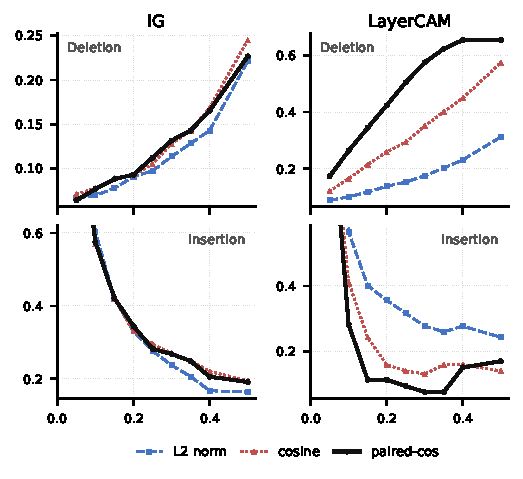
\includegraphics[width=0.76\linewidth]{figures/fig1_shape_2x2.pdf}
% 【中文·图1标题】形状归一化的干预曲线（EER($r$)/EER$_\text{base}$ 除以其极值），IG（左）与 LayerCAM（右）。上：删除；下：插入。IG 的三种目标曲线基本重叠：作为梯度方法它已在内部编码了判别方向，故其排序在不同目标下保持稳定（是因为已经对齐而非因为无响应）。LayerCAM 的曲线则散开，因为目标对齐注入了 CAM 重加权本身所缺乏的验证几何。
\caption{Shape-normalized intervention curves ($\EER(r)/\EER_{\mathrm{base}}$ divided by its extremum) for IG (left) and LayerCAM (right); top: deletion; bottom: insertion. IG's three objectives stay superimposed: as a gradient method it already encodes the discriminative direction internally, so its ranking is stable under the objective (invariant because already aligned).}
\label{fig:objshape}
\end{figure}

\subsection{Attribution Track}

% 实验设置说明
% 【中文】表~\ref{tab:attr} 报告主模型（Noise+SpecAug）上 4 算法 × 3 目标 × 双忠实度指标的完整比较，在整个测试集上评估；所有指标都相对基准 EER $2.87\%$ 归一化。
Table~\ref{tab:attr} reports the full comparison on the primary model (Noise+SpecAug); all metrics are normalized against the base EER of $2.76\%$.

% ---- Table 1：归因对比主表 ----
% 关键模式：同一算法内 cosine/paired-cos 统治 L2；LayerCAM+cosine 达到最优
\begin{table}[t]
\centering
% 【中文·表1标题】主模型上的归因忠实度（整个测试集，基准 EER $2.87\%$）。每列最优\textbf{加粗}。关键模式：将目标对齐到验证判决（L2 $\to$ cosine）提升了每一种算法，且 LayerCAM 在 cosine 目标下于两个指标上都达到最优忠实度。
\caption{Attribution faithfulness on the primary model (Noise+SpecAug, base EER $2.76\%$); best per column in \textbf{bold}.}
\label{tab:attr}
\small
\begin{tabular}{llcccc}
\toprule
\multirow{2}{*}{Alg.} & \multirow{2}{*}{Obj.} & \multicolumn{2}{c}{Discriminative} & \multicolumn{2}{c}{Representational} \\
\cmidrule(lr){3-4} \cmidrule(lr){5-6}
 & & Del $\uparrow$ & Ins $\downarrow$ & Del $\downarrow$ & Ins $\uparrow$ \\
\midrule
\multirow{3}{*}{IG}
  & L2         & 4.25 & 1.42 & 0.52 & 0.73 \\
  & cosine     & 4.55 & 1.21 & 0.49 & 0.76 \\
  & paired-cos & 4.48 & 1.25 & 0.51 & 0.75 \\
\midrule
\multirow{3}{*}{LayerCAM}
  & L2         & 3.70 & 1.21 & 0.52 & 0.76 \\
  & cosine     & 5.70 & 0.58 & \textbf{0.42} & \textbf{0.88} \\
  & paired-cos & \textbf{5.76} & \textbf{0.36} & 0.53 & 0.84 \\
\midrule
\multirow{3}{*}{Score-CAM}
  & L2         & 2.31 & 2.18 & 0.64 & 0.68 \\
  & cosine     & 3.71 & 1.50 & 0.54 & 0.72 \\
  & paired-cos & 4.97 & 0.79 & 0.52 & 0.75 \\
\midrule
\multirow{3}{*}{Guided IG}
  & L2         & 4.39 & 1.57 & 0.55 & 0.74 \\
  & cosine     & 4.50 & 1.43 & 0.54 & 0.76 \\
  & paired-cos & 4.64 & 1.52 & 0.53 & 0.75 \\
\midrule
\textit{Random} & --- & \textit{1.50} & \textit{1.72} & \textit{0.69} & \textit{0.66} \\ 
\bottomrule
\end{tabular}
\end{table}
% ---- Figure 2：提前到 §4.3 之前，让 LaTeX 浮到附近页顶 ----
\begin{figure*}[t]
\centering
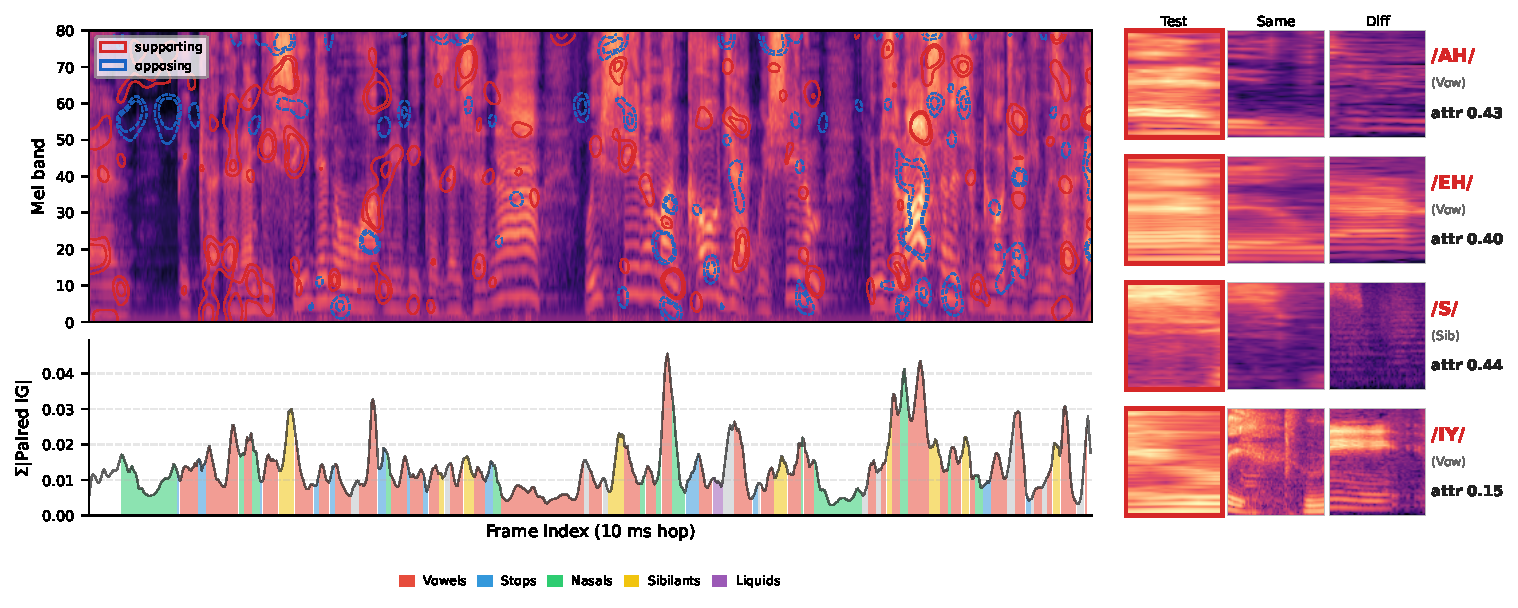
\includegraphics[width=0.82\textwidth]{figures/fig2_paired_ig_evidence.pdf}
% 【中文·图2标题】成对 IG 在梅尔谱上的符号解析显著性（Noise+SpecAug 模型）。红色轮廓 = 支持身份；蓝色 = 反对身份。下panel：逐帧 $\Sigma|\text{Paired IG}|$，按音素类着色。元音段主导了归因幅度。
\caption{Paired IG sign-resolved saliency on mel-spectrogram (Noise+SpecAug model). Red contours = identity-supporting; blue = identity-opposing. Lower panel: per-frame $\Sigma|\text{Paired IG}|$ colored by phoneme class; the per-phoneme values annotate this single illustrative utterance; class conclusions rest on full-test-set aggregation (Sec.~\ref{sec:framework}).}
\label{fig:paired_ig_vis}
\end{figure*}
% 核心发现：方向一致 + 幅度异质（先方向后幅度，消除矛盾感）
% 【中文】将目标从 L2 范数对齐到成对余弦，对全部四种算法都提升了判别性忠实度，但提升远非均匀（表~\ref{tab:attr}）：对 CAM 类方法显著，对梯度类方法则微弱。这一对齐可分解为两个阶段。第一阶段 L2$\to$cosine（去掉范数、匹配验证几何）是对每种算法都有帮助的一致正向分量。第二阶段 single$\to$paired cosine（加入冒充者项）随后以依赖算法的方式调节该增益，对前向扰动方法 Score-CAM 最强——其掩码重加权直接利用同/异对比；而梯度类方法已在内部编码判别方向，在 cosine 阶段就吸收了大部分目标几何，此后变化甚微。与此一致，Score-CAM 在失配的 L2 目标下于插入指标上跌破随机基线（表~\ref{tab:attr}）：目标失配可将排序推至随机水平以下，凸显目标对齐的效应真实存在、但以算法为条件。
Aligning the objective from the L2 norm toward the paired cosine improves discriminative faithfulness for all four algorithms, but the gain is far from uniform: substantial for CAM-based methods, marginal for gradient-based ones. The alignment factorizes into two stages. The first, L2$\to$cosine (removing the norm, matching the verification geometry), is the consistently positive component helping every algorithm. The second, single$\to$paired cosine (adding the impostor term), then modulates the gain algorithm-dependently, most strongly for Score-CAM, whose mask reweighting directly exploits the same/diff contrast, whereas gradient methods encode the discriminative direction internally and change little thereafter. Score-CAM under mismatched L2 even falls below random on insertion (Table~\ref{tab:attr})---misalignment can push a ranking below chance, so the alignment effect is real but algorithm-conditioned.



% 形状分析段
% 【中文】图~\ref{fig:objshape} 揭示了聚合 AUC 所掩盖的结构。形状归一化后，梯度类算法在其三种目标下基本重叠，而 CAM 类则散开，在两个方向上都如此。早期斜率行为（$r \leq 0.2$）讲述同样的故事：LayerCAM 的曲线在目标对齐下急剧分离，而 IG 的几乎不动。
Figure~\ref{fig:objshape} reveals structure that aggregate AUC hides: after shape normalization, gradient-based algorithms stay superimposed across their three objectives while CAM-based ones fan apart in both directions; the early slopes ($r\leq0.2$) tell the same story.

% 排序消融
% 【中文】一项排序规则消融确认，聚合必须尊重各算法的符号语义。CAM 重要度按构造非负~\cite{jiang2021layercam}，故 LayerCAM 用 $\sum \text{ReLU}(a)$ 聚合；若强行套用分类惯例 $\sum|a|$，则会混淆支持与反对证据，使删除指标从 $6.97$ 退化到 $2.91$。这是正确测量的前提，而非一个相互竞争的杠杆：一旦聚合与算法匹配，目标效应便清晰且可复现地显现。
An ablation confirms the aggregation must respect each method's sign semantics: applying the classification convention $\sum|a|$ to LayerCAM (non-negative by construction~\cite{jiang2021layercam}) conflates supporting and opposing evidence and degrades Del from $5.76$ to $2.48$, versus its native $\sum\text{ReLU}(a)$; with sign-matched aggregation the objective effect emerges cleanly and reproducibly.



% 符号解析可视化（去 subsection 标题，内联引导）
% 【中文】\textbf{符号解析可视化。}除聚合忠实度外，成对余弦目标独具\emph{符号解析}能力：正值标记"支持身份"、负值标记"反对身份"区域，故符号保持型算法（如 IG）产出图~\ref{fig:paired_ig_vis} 中的图（红=支持，蓝=反对）。无论 L2 范数 IG（其符号对验证无信息）还是 CAM 方法（无符号）都无法做出这一区分。
\textbf{Sign-resolved visualization.} Beyond aggregate faithfulness, the paired-cosine objective is uniquely \emph{sign-resolved}: positive values mark ``identity-supporting'' and negative ``identity-opposing'' regions, so sign-preserving algorithms such as IG yield Figure~\ref{fig:paired_ig_vis} (red/supporting, blue/opposing)---a distinction neither L2-norm IG nor unsigned CAM can make.


% ---- Table 2：提前到 §4.4 标题之前，让 LaTeX 浮到附近页顶 ----
% ---- Table 2：去 CI 后改为单栏 table（不再跨栏）----
\begin{table}[t]
\centering
% 【中文·表2标题】各训练条件下逐音素类的因果 $\dEER$（pp）（$\star$ = 主模型；EER 以 \% 计，Spec = SpecAug）。各列报告在整个 37{,}720 个 trial 上的均值。读法：SpecAug 与元音依赖的最大幅度下降相关联，且 MUSAN 的重塑效应大部分与 SpecAug 已诱导的部分重合。
\caption{Per-phoneme-class causal $\dEER$ (pp) across training conditions ($\star$ = primary; EER in \%, Spec = SpecAug); means over all 37{,}720 trials.}
\label{tab:prior}
\small
\setlength{\tabcolsep}{1.0pt}
\begin{tabular}{lcccccc}
\toprule
Model & EER & Vowel & Plos. & Nasal & Fric. & Liq. \\
\midrule
Clean              & 3.92 & $+10.06$ & $+0.57$ & $+0.51$ & $+0.45$ & $+0.06$ \\
SpecAug            & 3.44 & $+2.62$  & $+0.13$ & $+0.08$ & $+0.00$ & $+0.03$ \\
Noise              & 2.99 & $+7.08$  & $+0.38$ & $+0.34$ & $+0.32$ & $+0.08$ \\
Noise+Spec$^\star$ & 2.87 & $+2.13$ & $+0.25$ & $+0.23$ & $+0.16$ & $+0.10$ \\
Noise+Spec+Adv     & 2.76 & $+1.72$  & $+0.11$ & $+0.12$ & $+0.12$ & $-0.01$ \\
\bottomrule
\end{tabular}
\end{table}

\subsection{Prior Track: Training Strategy Reshapes Phoneme Reliance}

% Table 2 引用
% 【中文】表~\ref{tab:prior} 报告五个训练条件下逐音素类的因果 $\dEER$（pp）。


% 2×2 因子化分析
% 【中文】把元音列对照 $2\times2$ 的 MUSAN $\times$ SpecAug 因子设计来读：单独 SpecAug 大幅降低元音的因果贡献，单独 MUSAN 降低得少得多，而在 SpecAug 之上再加 MUSAN 只带来边际变化；该因子模式将重塑的主要份额与 SpecAug 关联起来。然而 MUSAN 在 SpecAug 之上仍改善基准 EER：性能增益与信息使用的重塑不必同时发生。重塑集中在元音类——非元音类数值很小，仅作定性解读。
Reading the vowel column against the $2\times2$ MUSAN $\times$ SpecAug factorial, SpecAug alone sharply reduces the causal vowel contribution, MUSAN alone far less, and MUSAN on top of SpecAug only marginally; the factorial pattern associates SpecAug with the dominant share of the reshaping. Yet MUSAN still improves the base EER on top of SpecAug: performance gain and information-usage reshaping need not coincide; the reshaping concentrates in vowel.

% 混淆排除
% 【中文】为排除明显的混淆，随机预算插入产生的元音 EER 为 4.32\%，对比随机预算基线 $4.74 \pm 0.06$\%，排除了时长混淆；而用粉噪声替代零掩蔽得到元音 $\dEER = +3.18$ pp（对比 $+2.13$ pp），方向一致，排除了零值 OOD 伪影。
Two controls rule out obvious confounds: random-budget insertion yields vowel EER 4.32\% versus a $4.74\pm0.06$\% random baseline (no duration confound), and pink-noise masking yields vowel $\dEER = +3.18$ pp versus $+2.13$ pp for zeroing (no OOD artifact).

% τ = 1.0 的报告（并入 §4.4，去 subsection 头；加 run-in 引导）
% 【中文】取 cosine 目标下的 LayerCAM，逐帧显著性聚成五类得 R_attr，与因果排序 R_prior 比较：元音类在观察性归因与因果干预下都居首，其余类方向一致——跨轨相互印证，说明归因追踪的是判决依据。
\textbf{Cross-track consistency.} Taking LayerCAM with the cosine objective (best representational in Table~\ref{tab:attr}), we aggregate its per-frame saliency into the five phoneme classes to obtain $R_{\text{attr}}$, compared against the causal ranking $R_{\text{prior}}$: the vowel class ranks foremost in both, the rest agree in direction---cross-track corroboration that the attribution tracks the model's decision basis.

% ========================================================================
% §4 讨论与结论（合并，避免重复）
% ========================================================================
\section{Discussion and Conclusion}
\label{sec:disc}

% Discussion 两段并一段：两层结构 + 结论一句话 + future work
% 【中文】目标对齐两层结构：L2→cosine 帮全部四算法，paired 依赖算法。总之帧干预统一 SV 可解释性评估（objective 作受控变量、判别/表征忠实度分离），揭示训练诱导的音素依赖；多骨干/基准是未来方向。
Objective alignment has a two-level structure: the L2 $\to$ cosine stage improves discriminative faithfulness for every attribution algorithm, whereas the further step from single to paired cosine is algorithm-dependent, substantially aiding CAM-based methods but barely gradient-based ones. Frame intervention unifies SV interpretability evaluation---the attribution objective as a controlled variable, with dual faithfulness metrics separated---and reveals training-induced phoneme reliance invisible to standard EER. Our conclusions are drawn on a single ECAPA-TDNN backbone and the VoxCeleb1-O easy protocol; other backbones and benchmarks are future work.

% ========================================================================
% 参考文献
% ========================================================================
% 参考文献（正常字号）
% 参考文献（正常字号；\balance 平衡末页两栏）
\balance
\bibliographystyle{IEEEbib}
\bibliography{refs}

\end{document}
